


\begin{figure}[!htb]
\caption{Incidence of COVID-19 cases in the HUS area by age group and language during the first wave of the epidemic in 2020, for Finnish (fi), Swedish (sv), English (en), Russian (ru) and other language groups.}
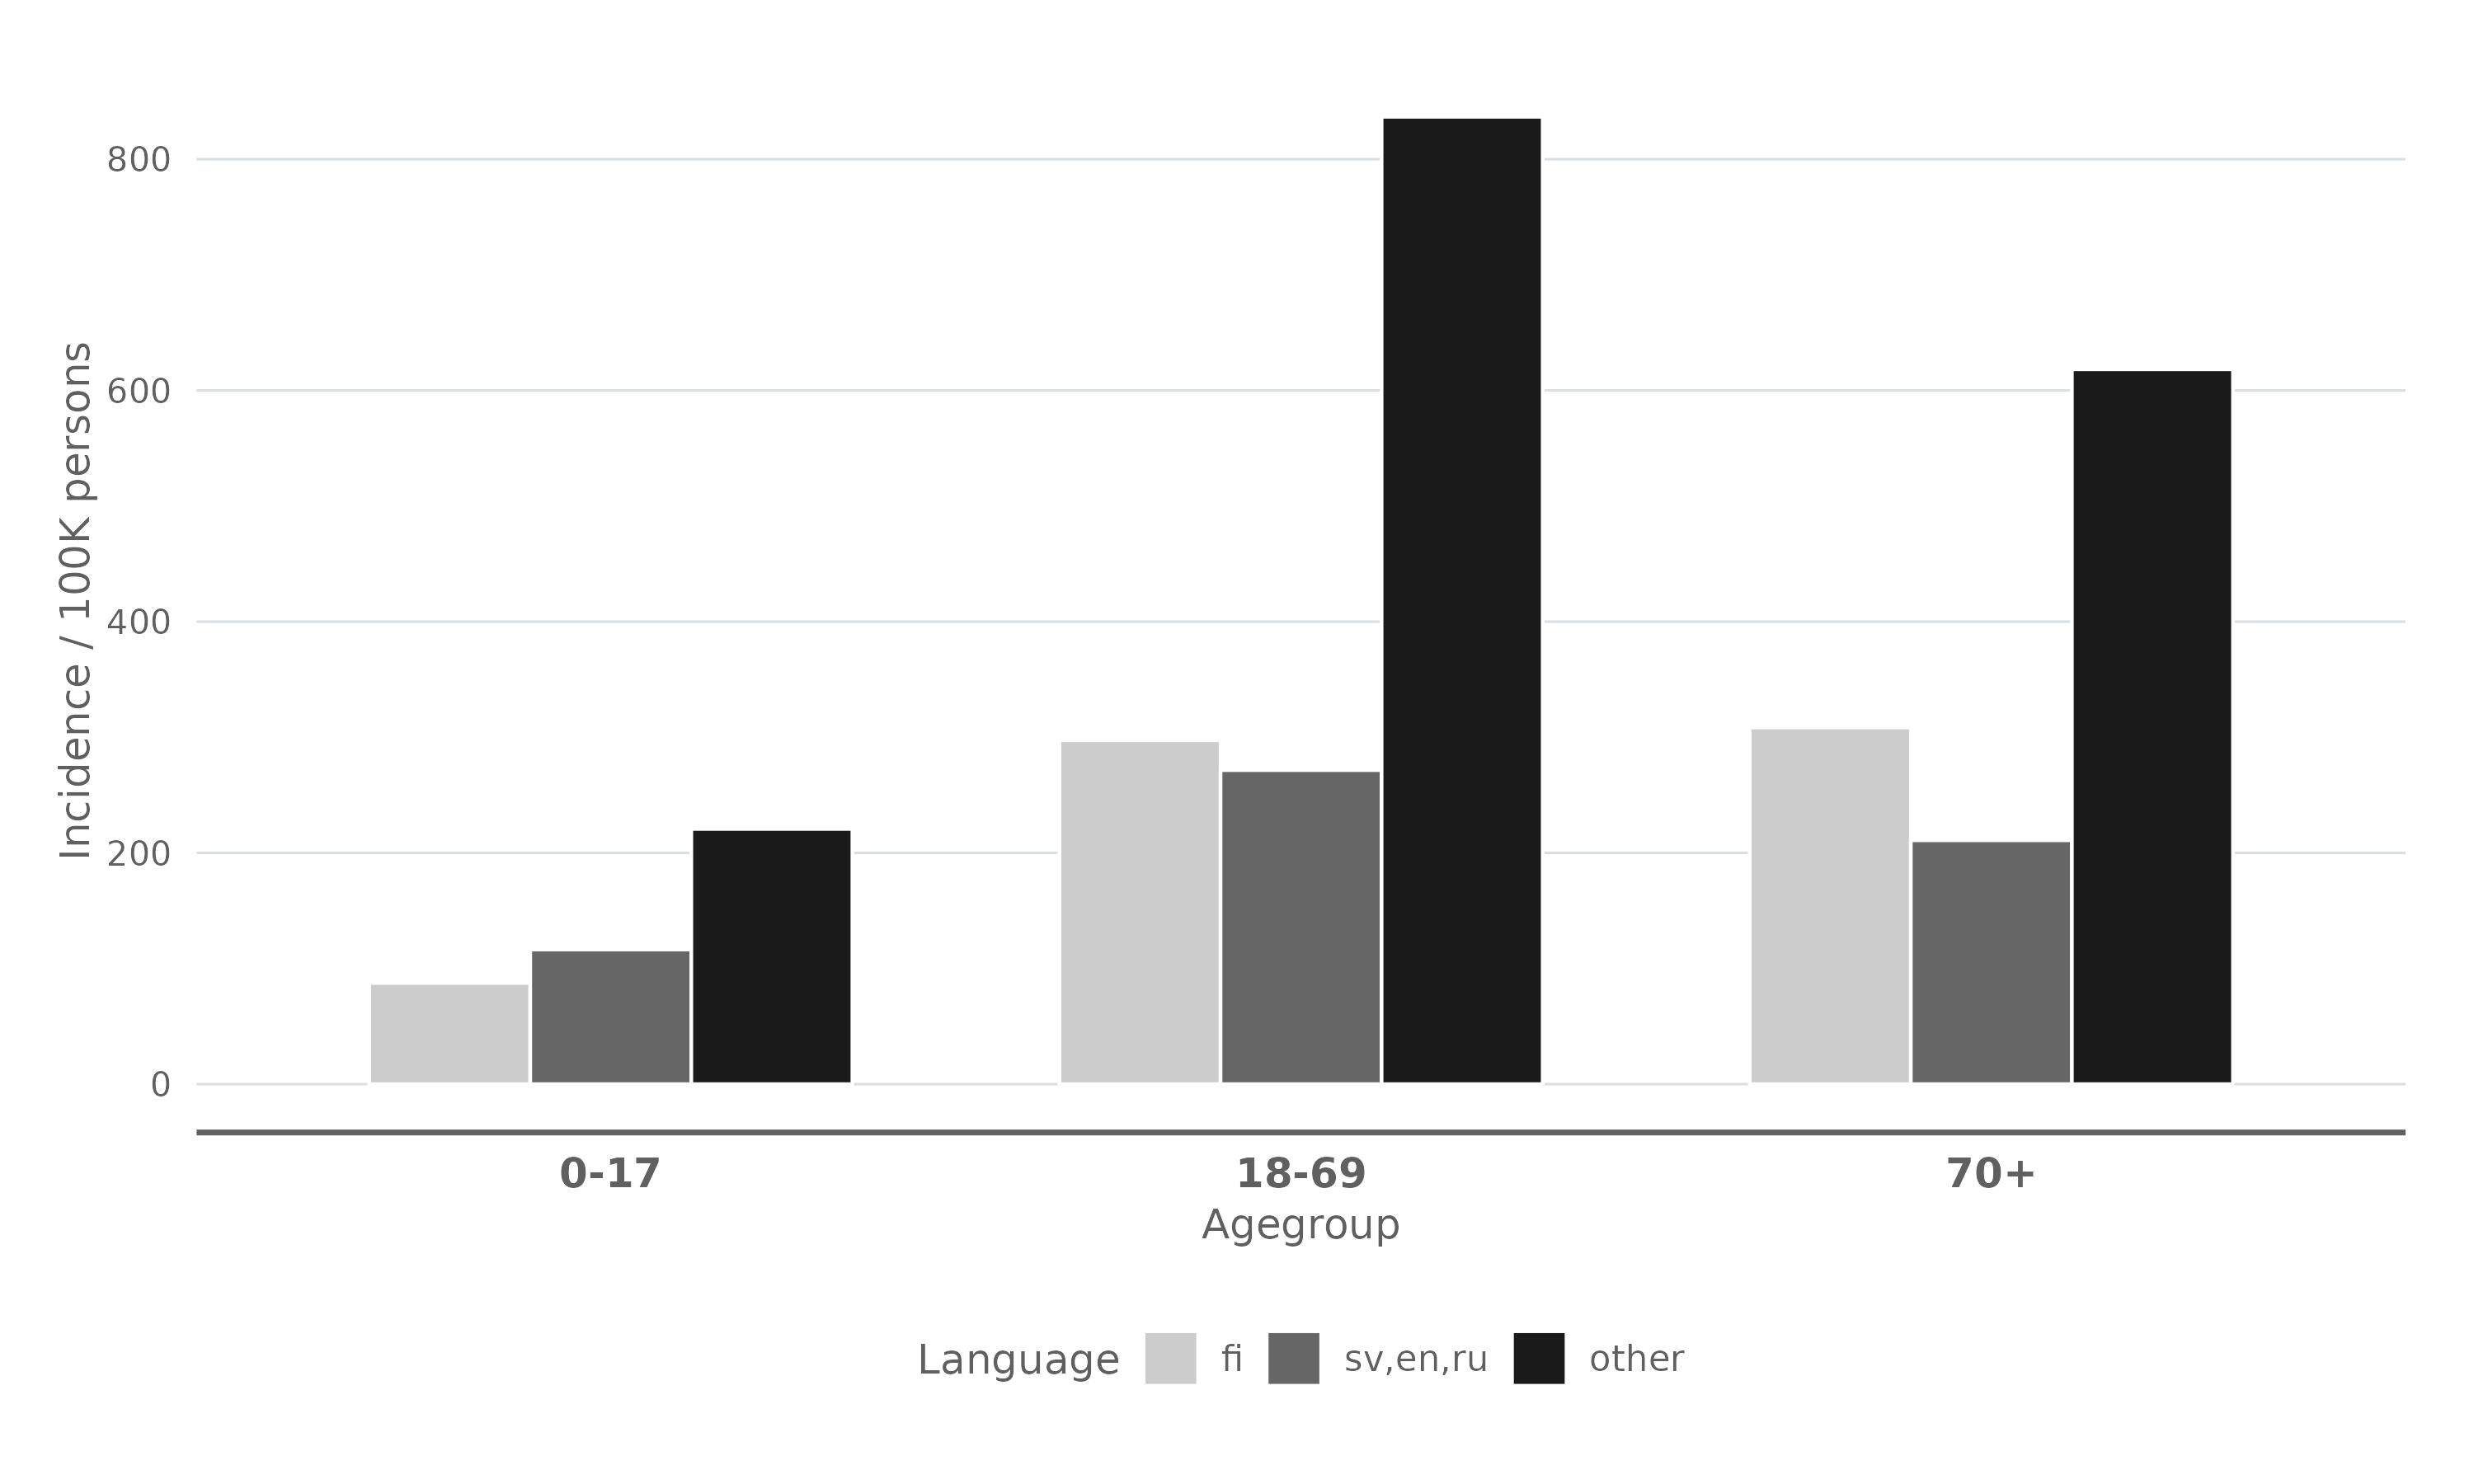
\includegraphics[width=\linewidth]{img/ttr_incidence_lang_bar.png}
\label{fig:incidence_lang}
\end{figure}


\newpage



\begin{figure}[!htb]
\caption{Age distributions of: population in the extended capital region of Finland at the end of 2021 (HUS); COVID-19 cases for the HUS population during the first wave of the COVID-19 epidemic in 2020; the study population, i.e. the target population of the current study (HUS (incl.)); COVID-19 cases from the study population during the first wave of the COVID-19 epidemic in 2020 (FNIDR (incl.)); serological survey participants from the study population during the first wave (Serosurveys).}
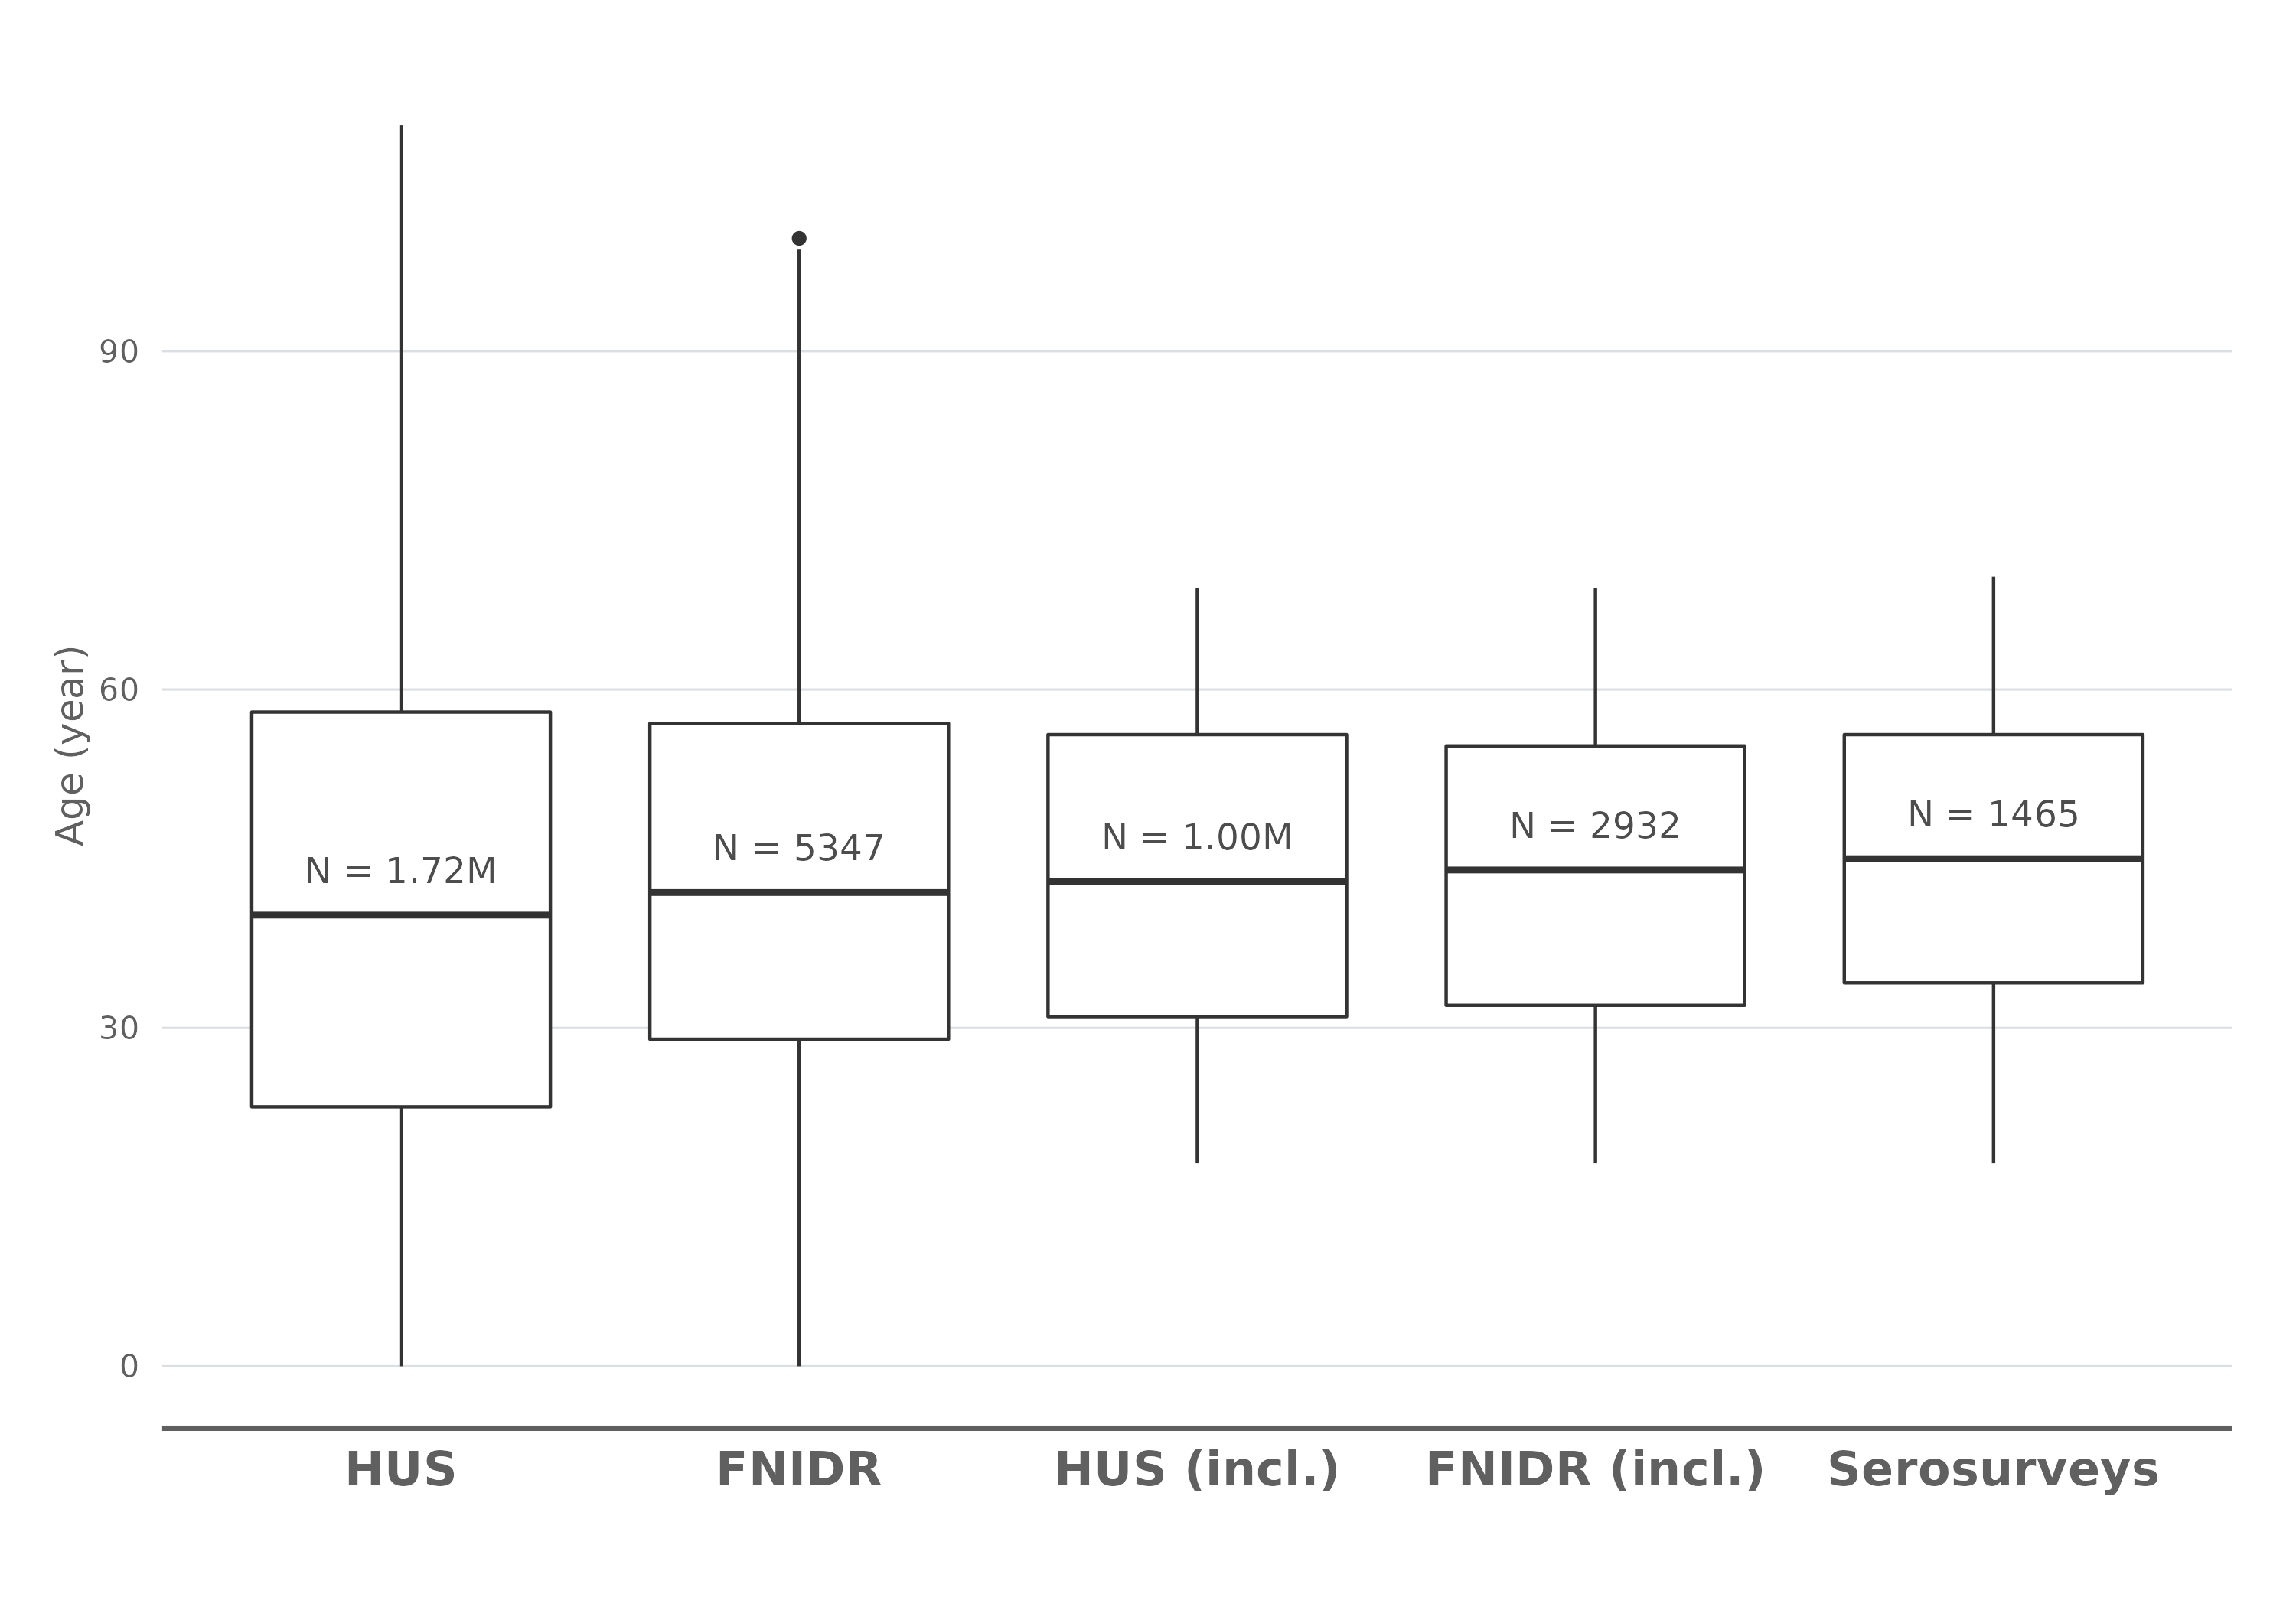
\includegraphics[width=\linewidth]{img/pop_ttr_sero_age_box.png}
\label{fig:pop_ttr_sero}
\end{figure}


\newpage



\begin{figure}[!htb]
\centering


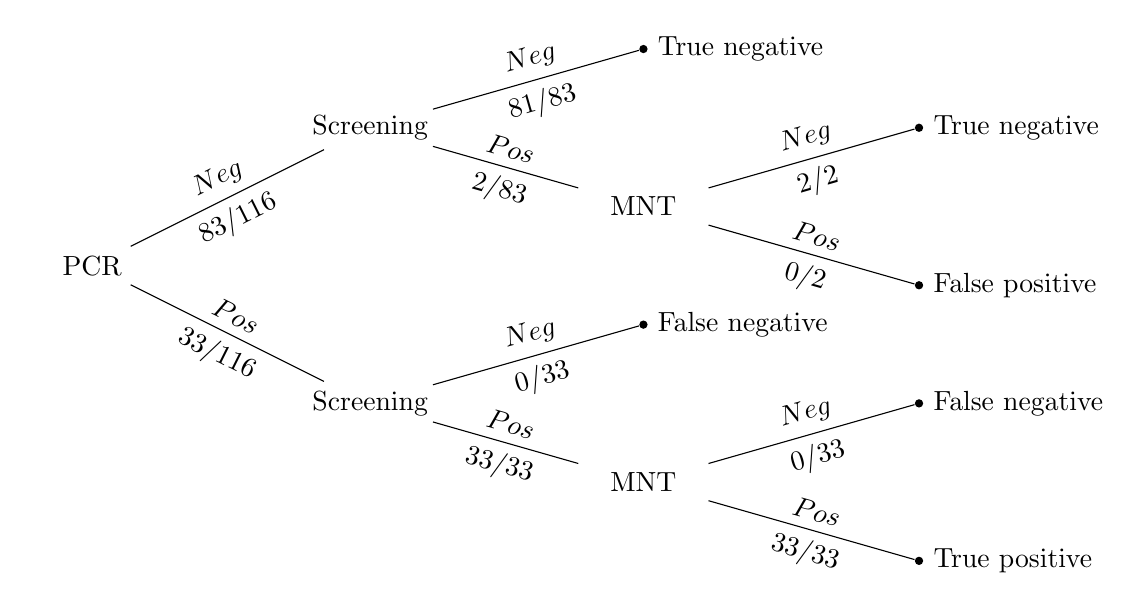
\begin{tikzpicture}[grow=right, sloped]

% Set the overall layout of the tree
\tikzstyle{level 1}=[level distance=3.5cm, sibling distance=3.5cm]
\tikzstyle{level 2}=[level distance=3.5cm, sibling distance=2cm]

% Define styles for bags and leafs
\tikzstyle{bag} = [text width=4em, text centered]
\tikzstyle{end} = [circle, minimum width=3pt,fill, inner sep=0pt]

% Builds from bottom to top
\node[bag] {PCR}
    child {
        node[bag] {Screening}        
            child {
                 node[bag] {MNT} 
                    child {
                        node[end, label=right: True positive] {}
                        edge from parent
                        node[above] {$Pos$}
                        node[below] {$33 / 33$}
                    } 
                    child {
                        node[end, label=right: False negative] {}
                        edge from parent
                        node[above] {$Neg$}
                        node[below] {$0 / 33$}
                    }
                edge from parent
                node[above] {$Pos$}
                node[below] {$33 / 33$}
            }
            child {
                node[end, label=right: False negative] {}
                edge from parent
                node[above] {$Neg$}
                node[below] {$0 / 33$}
            }
            edge from parent 
            node[above] {$Pos$}
            node[below] {$33 / 116$}
    }
        child {
        node[bag] {Screening}        
            child {
                 node[bag] {MNT} 
                    child {
                        node[end, label=right: False positive] {}
                        edge from parent
                        node[above] {$Pos$}
                        node[below] {$0 / 2$}
                    } 
                    child {
                        node[end, label=right: True negative] {}
                        edge from parent
                        node[above] {$Neg$}
                        node[below] {$2 / 2$}
                    }
                edge from parent
                node[above] {$Pos$}
                node[below] {$2 / 83$}     
            }
            child {
                node[end, label=right: True negative] {}
                edge from parent
                node[above] {$Neg$}
                node[below] {$81 / 83$}
            }
            edge from parent 
            node[above] {$Neg$}
            node[below] {$83 / 116$}
    };
\end{tikzpicture}
\caption{The antibody tests and their performances on the calibration data. The screening test is the result of the IgG antibody test, which may give false positive results. The confirmation test is a combination of the IgG and microneutralization tests (MNT), where the IgG positive samples are tested again with the MNT. After optimizing performance on the calibration data, which includes samples from PCR positive and negative individuals, the sensitivity and specificity of the screening test are 33/33 (100\%) and 81/83 (97.59\%), respectively, while the sensitivity and specificity of the confirmation test are 33/33 (100\%) and 83/83 (100\%), respectively.} 
\label{fig:labmethod}
\end{figure}


\newpage



\begin{figure}[!htb]
\centering
\caption{Prior mean, and 2.5\% and 97.5\% quantiles for each weekly seroprevalence $\pi^{(0)}_w$ in the Estimation model. The estimates were computed based on 40000 samples generated from the prior distribution of $\mathbf{\pi}$, see equation \ref{eq:model1_prior}. The model parameter values used in the simulation are given in Table \ref{tab:priors}. The sampling algorithm is described under Section \ref{seq:estimation}}. 
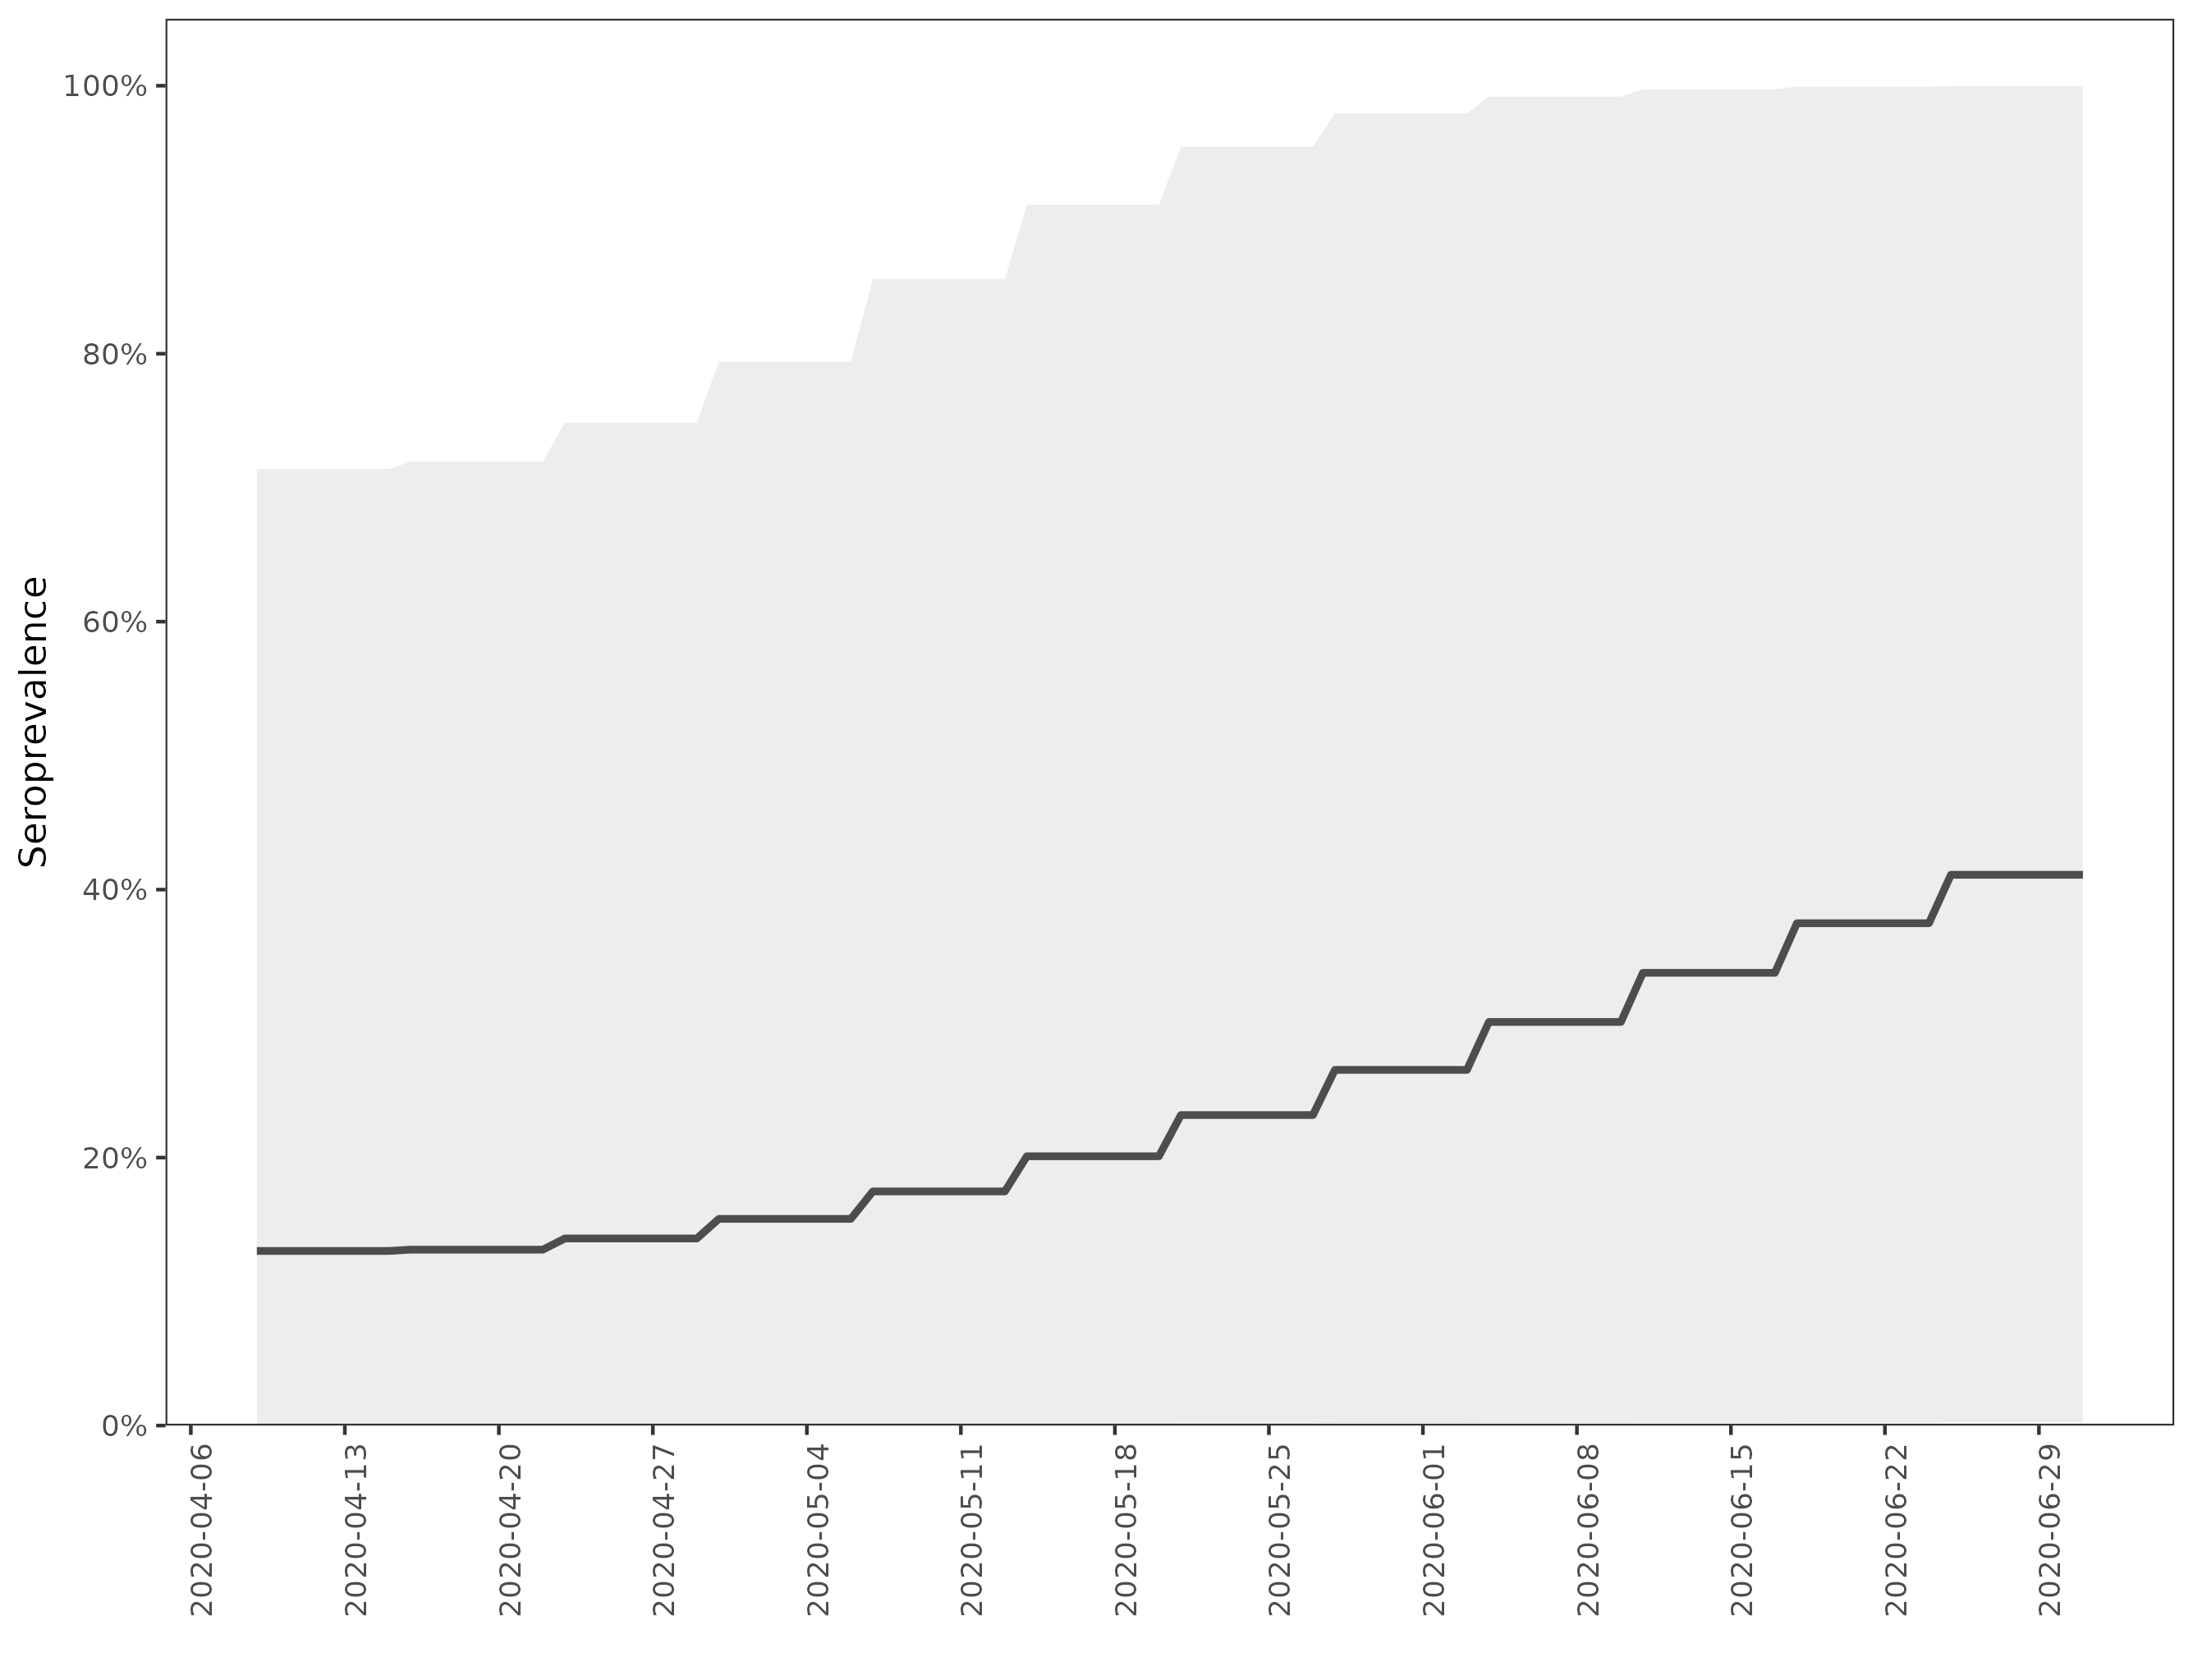
\includegraphics[width=\linewidth]{img/seroprevalence_prior.png} 
\label{fig:seroprevalence_prior}
\end{figure}


\newpage



\begin{figure}[!htb]
\centering
\caption{Posterior distributions for $\mu_U$ and $\sigma_U$ (see equation \ref{eq:model2_post}) and the posterior predictive distribution for $U$, the time from COVID-19 symptom onset to seroconversion. The distribution for $\mathbf{\theta} = (\mu_U, \sigma_U)$ was obtained by sampling as described in section \ref{seq:estimation}. The distribution for $U$ was obtained by sampling from the lognormal distribution using samples from the posterior distribution for $\mathbf{\theta}$. }

\begin{subfigure}{0.32\textwidth}
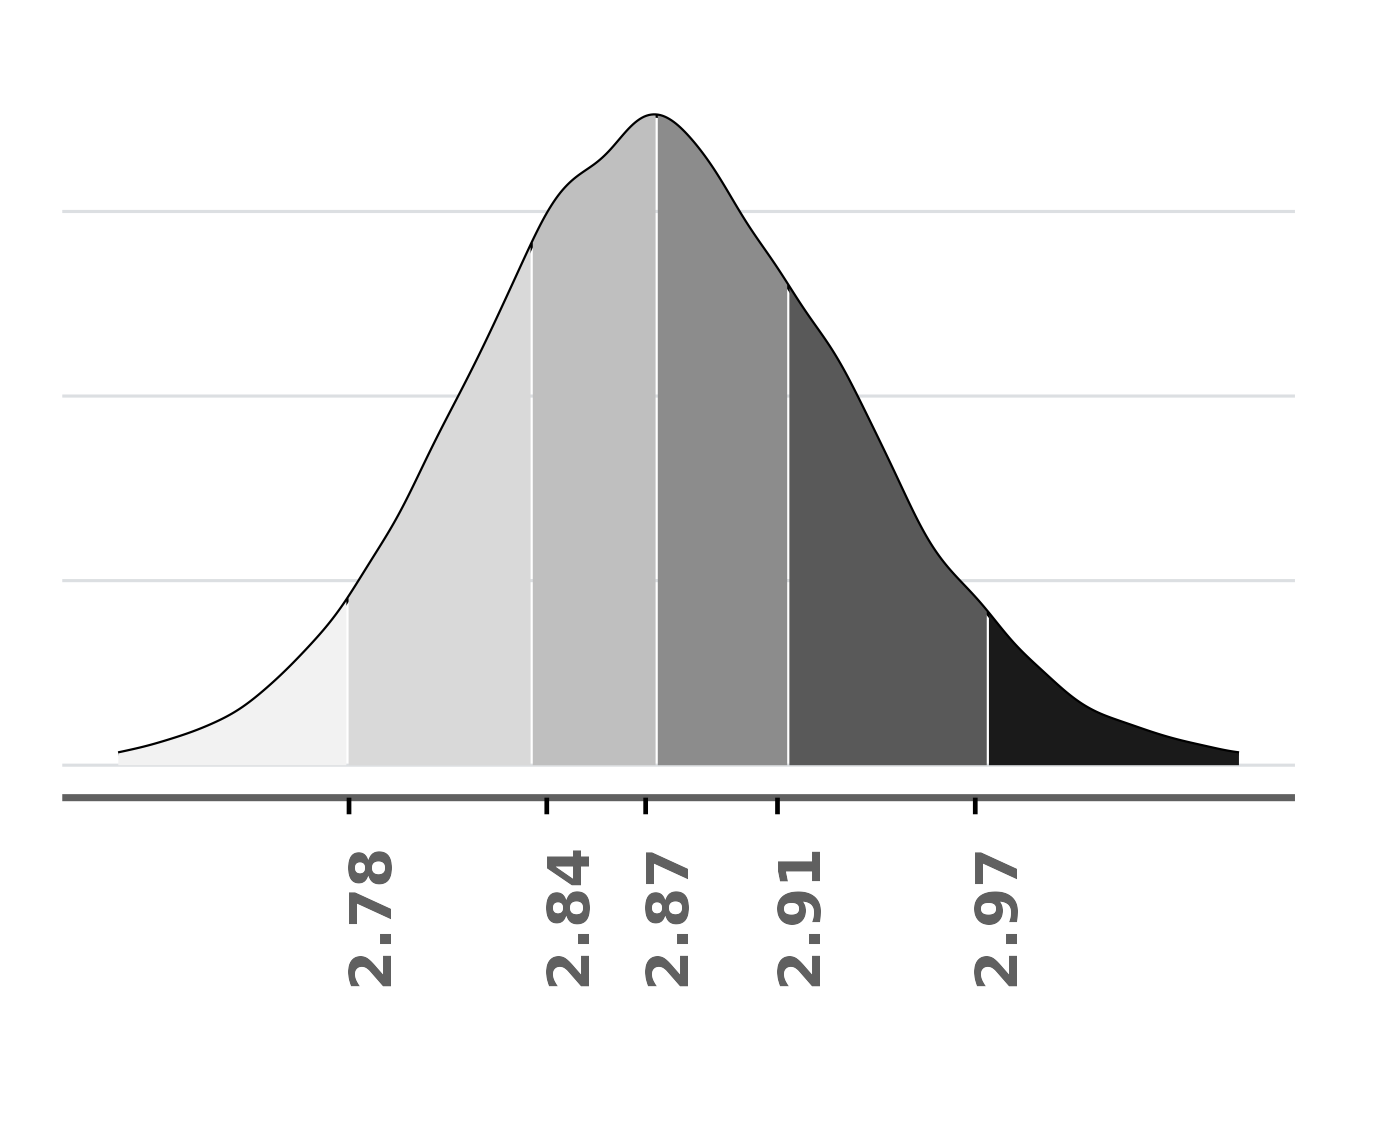
\includegraphics[width=\linewidth]{img/tan_mu.png} 
\caption{Posterior distribution of $\mu_U$} \label{fig:tan_mu}
\end{subfigure}%
\hspace*{\fill} 
\begin{subfigure}{0.32\textwidth}
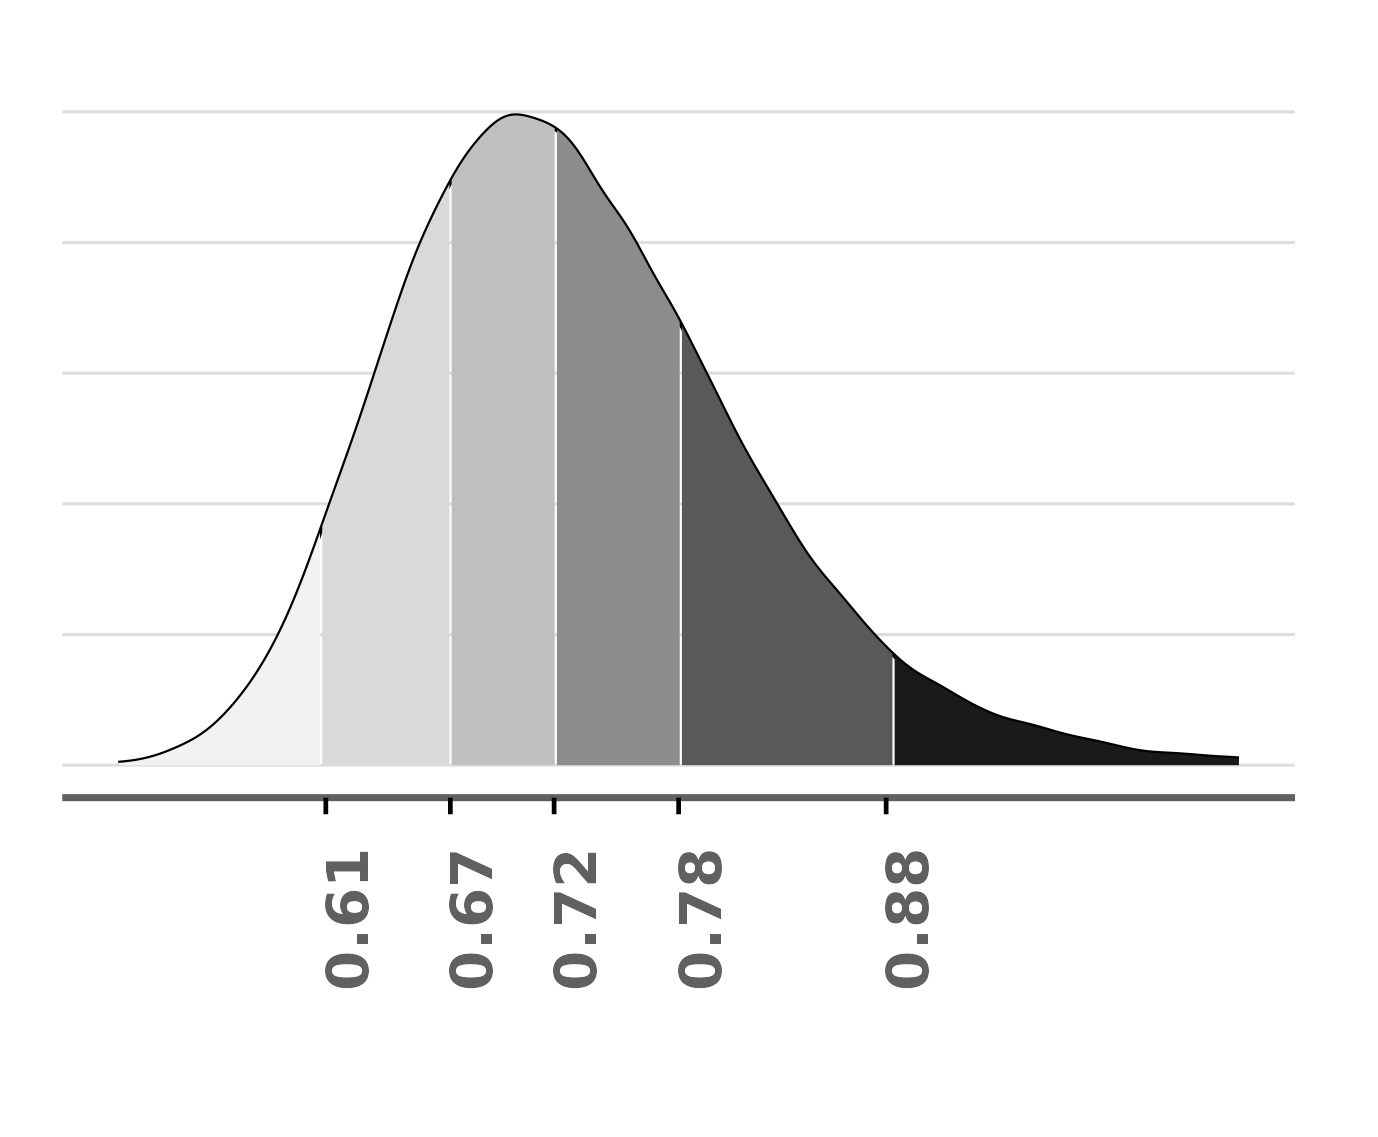
\includegraphics[width=\linewidth]{img/tan_sigma.png}
\caption{Posterior distribution of $\sigma_U$} \label{fig:tan_sigma}
\end{subfigure}%
\hspace*{\fill} 
\begin{subfigure}{0.32\textwidth}
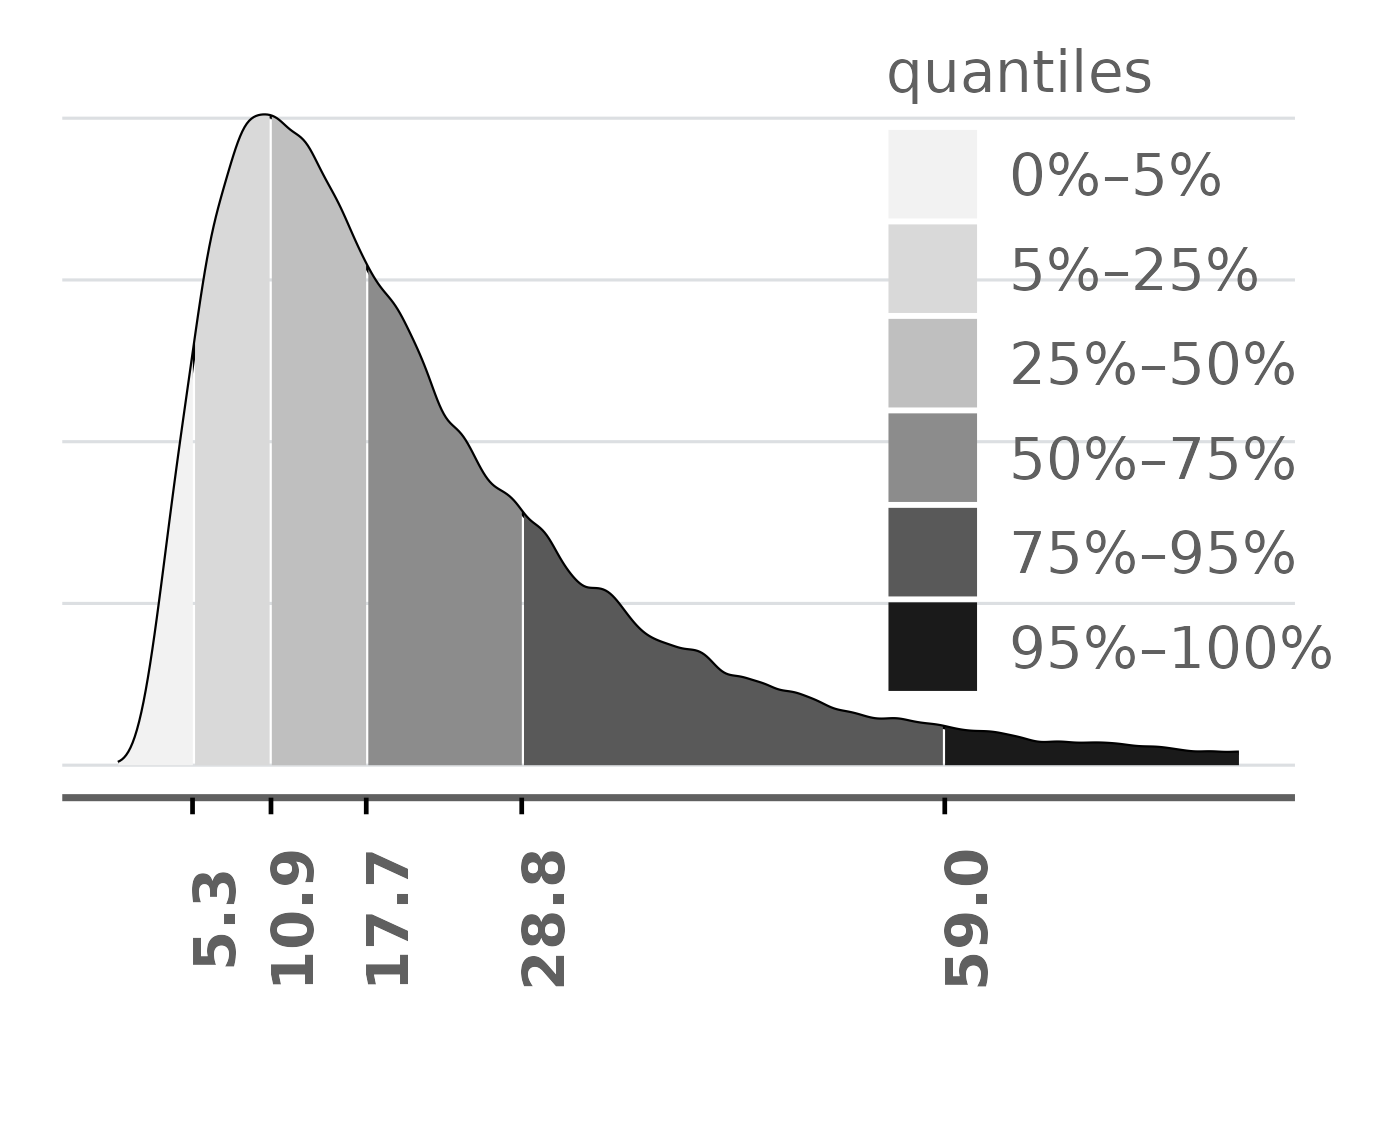
\includegraphics[width=\linewidth]{img/tan_lognorm.png}
\caption{Posterior predictive distribution of $U$.} \label{fig:tan_lognorm}
\end{subfigure}

\label{fig:U_posteriors}

\end{figure}



\newpage



\begin{figure}[!htb]
\centering
\caption{Prior and posterior distributions of the parameter $\sigma$, specified in equation \ref{eq:model1_prior}. Figure (a) shows the prior distribution. The posterior distributions were estimated separately using the confirmation test data (b) and the screening test data (c).}

\hspace*{\fill} 
\begin{subfigure}{0.3\textwidth}
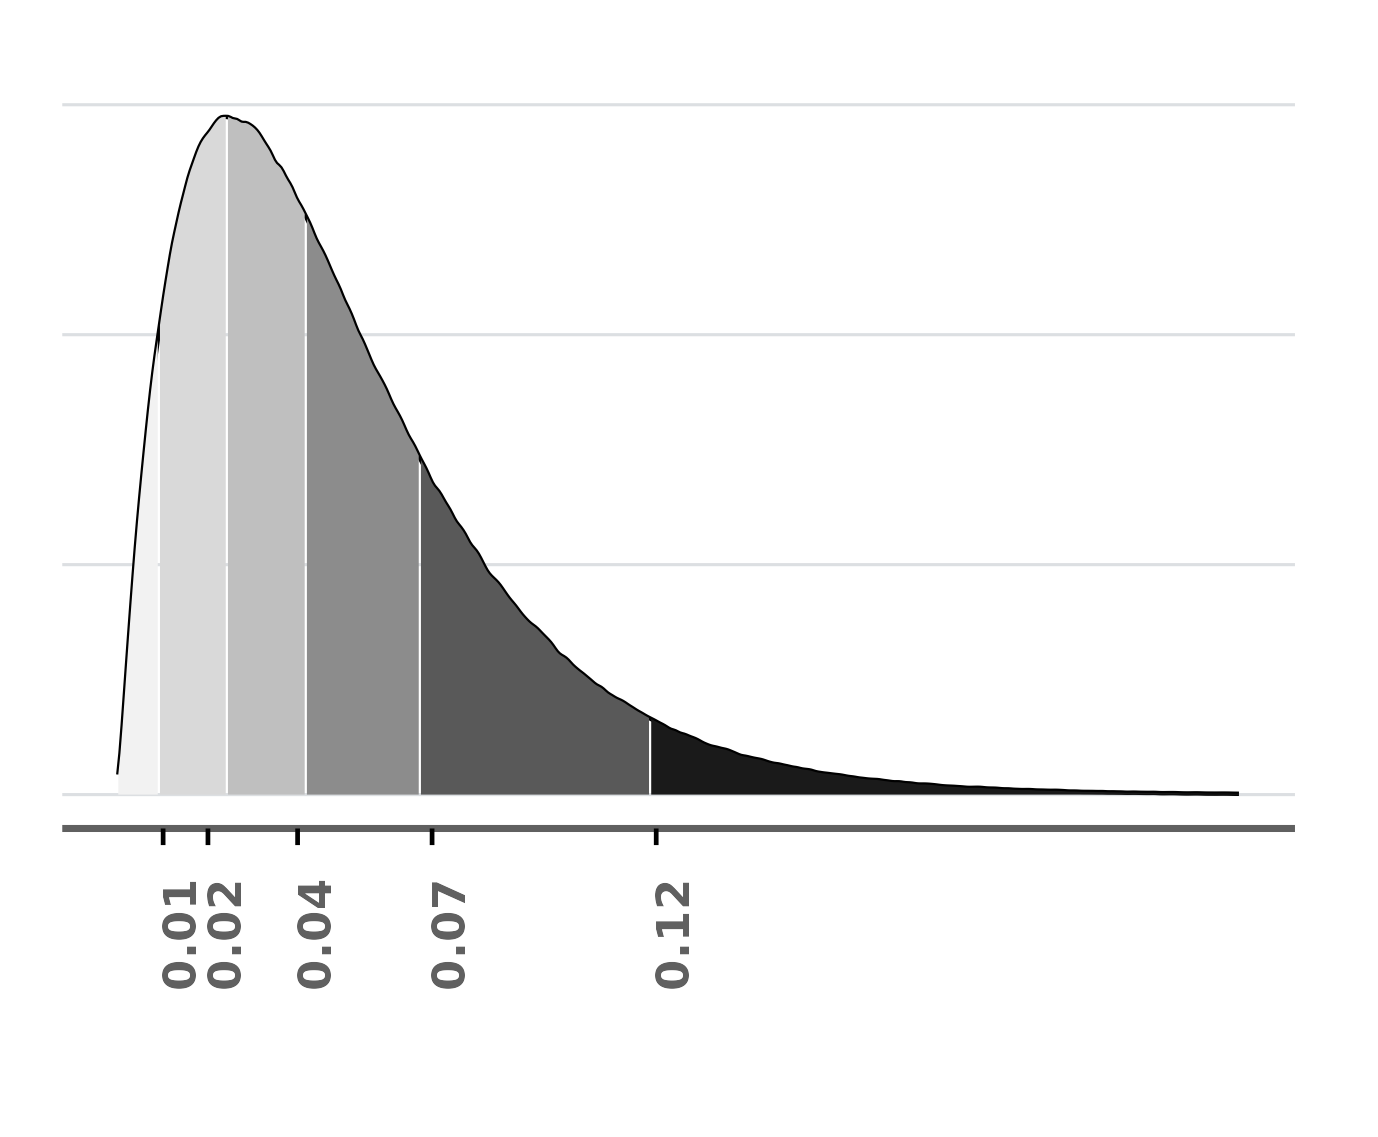
\includegraphics[width=\linewidth]{img/sero_sigma_prior.png}
\caption{Prior density for $\sigma$.} \label{fig:sero_sigma_prior}
\end{subfigure}%
\hspace*{\fill} 
\begin{subfigure}{0.3\textwidth}
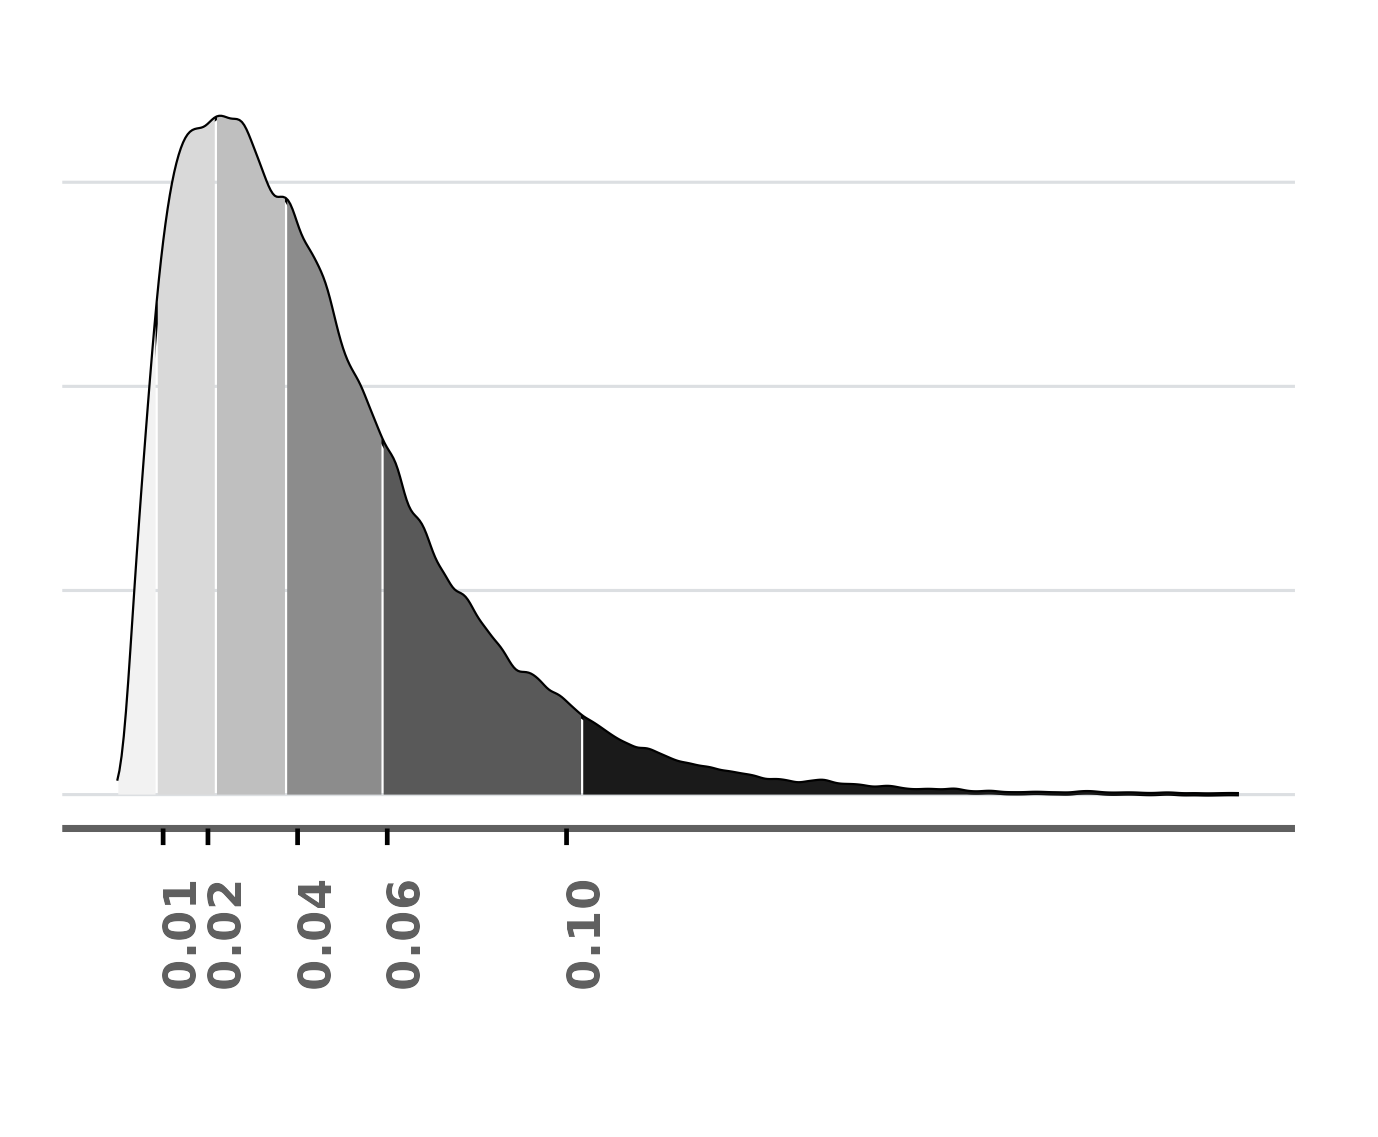
\includegraphics[width=\linewidth]{img/sero_sigma.png}
\caption{Posterior density for $\sigma$, estimated using the confirmation test data.} \label{fig:sero_sigma_mnt}
\end{subfigure}%
\hspace*{\fill} 
\begin{subfigure}{0.3\textwidth}
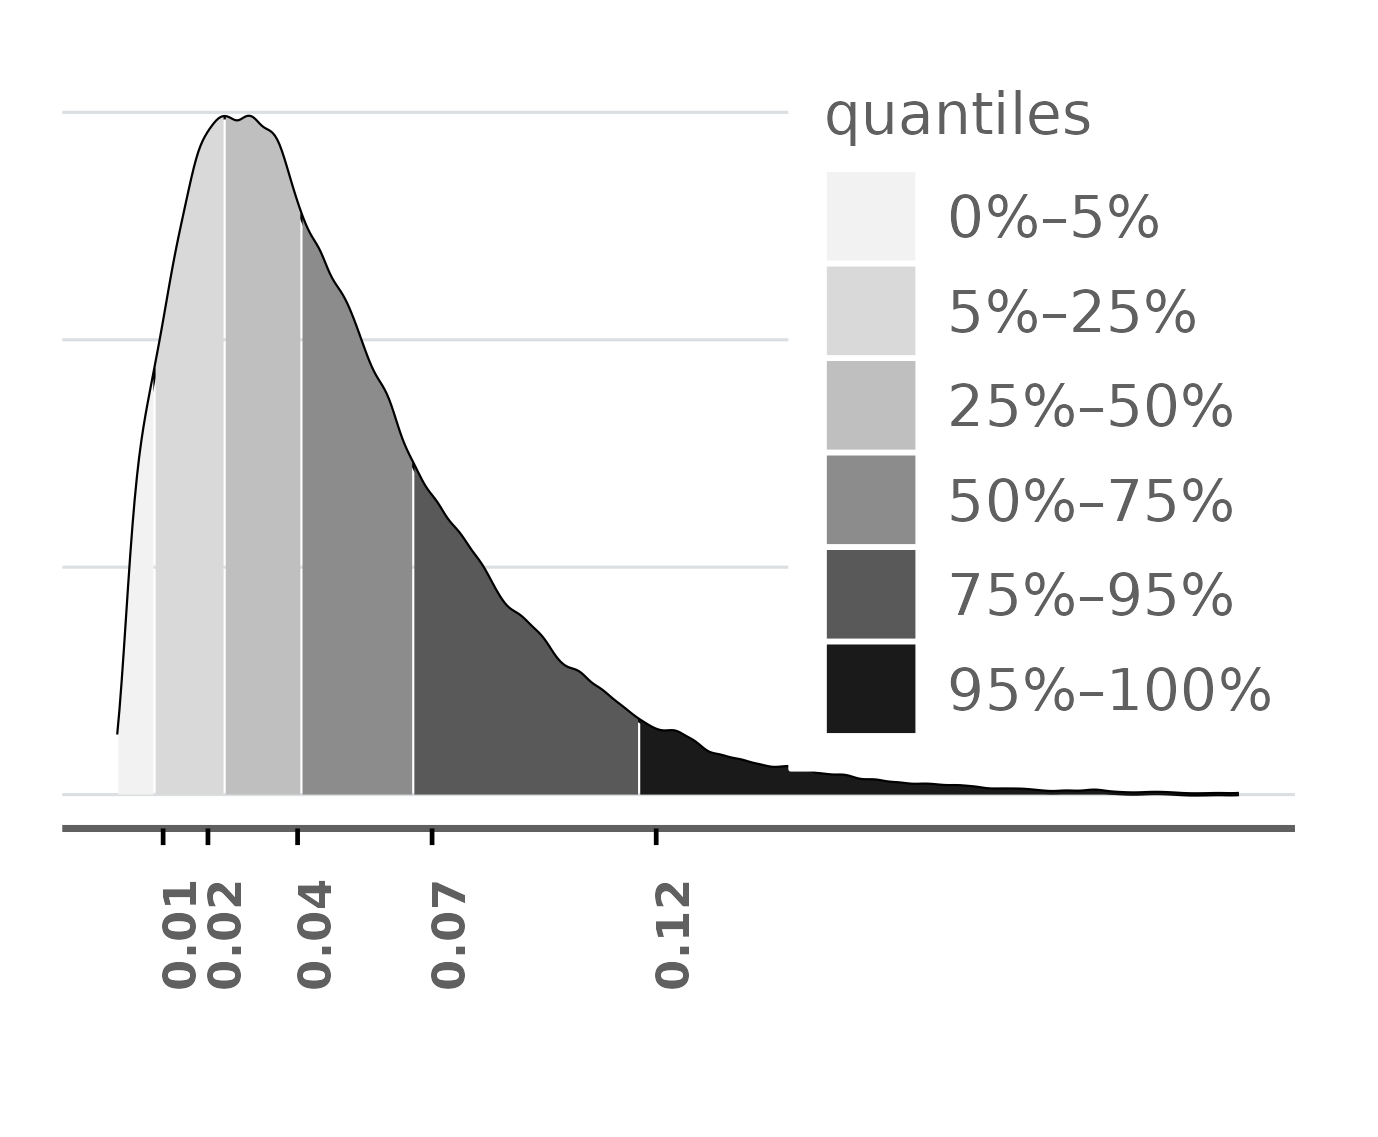
\includegraphics[width=\linewidth]{img/sero_sigma_screen.png}
\caption{Posterior density for $\sigma$, estimated using the screening test data.} \label{fig:sero_sigma_screen}
\end{subfigure}
\hspace*{\fill} 
\label{fig:sigma_posteriors}

\end{figure}

\newpage


\begin{figure}[!htb]
\caption{Age distribution of COVID-19 cases in the extended capital region of Finland during the first wave of the COVID-19 epidemic in 2020.}
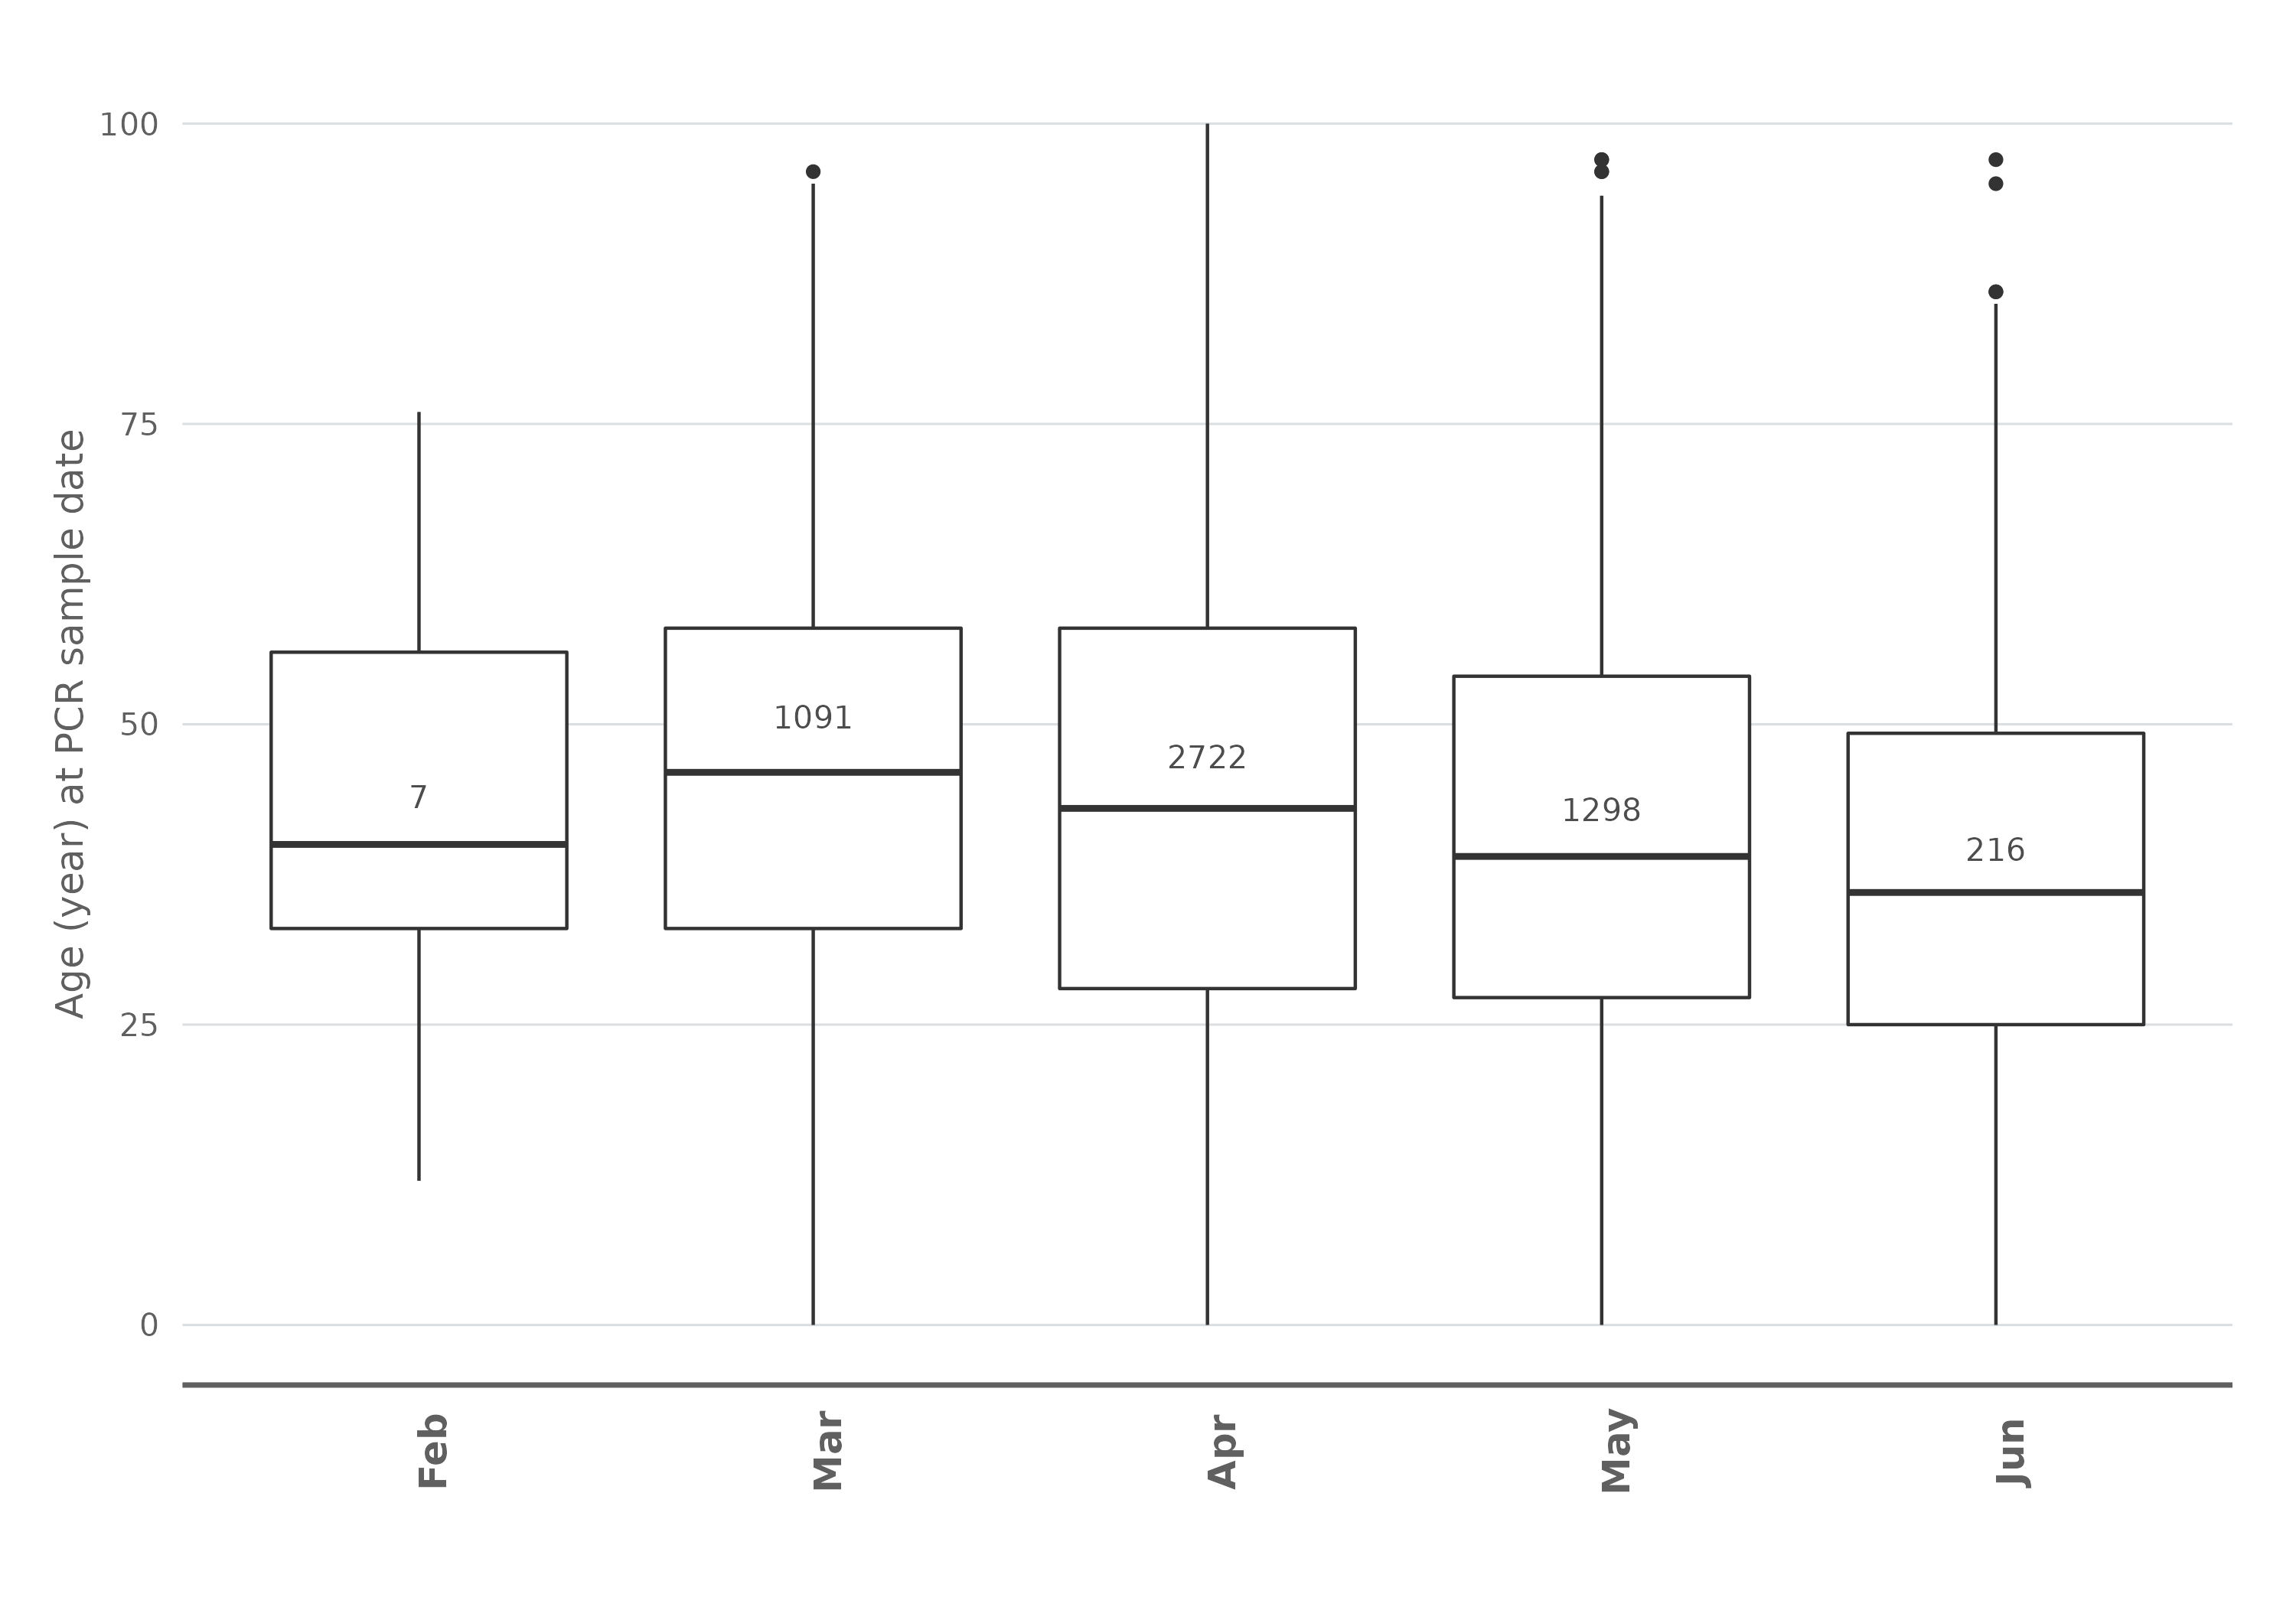
\includegraphics[width=\linewidth]{img/ttr_age_month_box.png} 
\label{fig:incidence_age}
\end{figure}

\newpage
